\documentclass[12pt,a4paper]{article}

\usepackage[margin=1in]{geometry}
\usepackage{graphicx}
\usepackage{amsmath}
\usepackage{amssymb}
\usepackage{booktabs}
\usepackage{hyperref}
\usepackage{xcolor}
\usepackage{float}
\usepackage{caption}
\usepackage{subcaption}

\hypersetup{
    colorlinks=true,
    linkcolor=blue!50!black,
    urlcolor=blue!50!black,
    citecolor=blue!50!black
}

\setlength{\parindent}{0pt}
\setlength{\parskip}{0.7em}
\setlength{\tabcolsep}{8pt}
\setlength{\emergencystretch}{2em}
\renewcommand{\arraystretch}{1.2}

\title{Padding Oracle Attacks on CBC Mode\\\large Theory, POODLE, and a Python Demonstration}
\author{Intro to Cryptography Project Report}
\date{March 2026}

\begin{document}

\hypersetup{pageanchor=false}
\begin{titlepage}
    \centering
    \vspace*{2.8cm}
    {\Huge \bfseries Padding Oracle Attacks on CBC Mode\par}
    \vspace{2cm}

    {\large Intro to Cryptography Project Report\par}
    \vspace{1.2cm}

    \begin{tabular}{ll}
        \textbf{Course:} & Intro to Cryptography \\
        \textbf{Topic:} & Padding Oracle Attacks on CBC Mode \\
        \textbf{Group Number:} & 8 \\
    \end{tabular}

    \vspace{1.2cm}

    {\large \textbf{Group 8 Members}\par}
    \vspace{0.5cm}

    \begin{tabular}{ll}
        Jeetrajsinh Gohil & 202303017 \\
        Kaushal Nandaniya & 202303036 \\
        Rom Tala & 202303051 \\
        Param Savjani & 202303046 \\
        Dhruvil Patel & 202301035 \\
        Tirth Kansagra & 202303055 \\
        Aryan Rathod & 202301164 \\
        Bhensdadia Vasu & 202301416 \\
        Zeel Dadhaniya & 202303010 \\
        Khush Patel & 202301142 \\
    \end{tabular}
\end{titlepage}
\hypersetup{pageanchor=true}

\begin{abstract}
Cipher Block Chaining (CBC) was widely used in network protocols and application-layer encryption before authenticated encryption became standard. By itself, CBC only gives confidentiality against passive observation. Once an attacker can modify ciphertext and learn even one bit about the result of decryption, for example whether PKCS\#7 padding is valid, the attacker can recover plaintext block by block without learning the secret key. This report explains CBC mode, padding validation, the chosen-ciphertext setting, and the byte-recovery mathematics behind padding oracle attacks. It then studies POODLE as the main case study, clarifies why it is historically important, and distinguishes that real-world protocol attack from a simplified local Python demonstration. The report closes with defenses, current industry practice, and the main lessons that motivate the use of authenticated encryption in modern systems.
\end{abstract}

\tableofcontents
\clearpage

\section{Introduction and Project Objective}

Block ciphers operate on fixed-size blocks, so practical systems need a mode of operation to encrypt messages of arbitrary length. CBC mode became one of the most widely deployed solutions because it is simple, efficient, and easy to implement with existing block ciphers such as AES. For many years CBC appeared to be a reasonable default choice for secure communication, especially in transport protocols and application-layer systems that needed confidentiality.

However, confidentiality alone is not enough when an attacker can actively interfere with the communication channel. If the receiver decrypts a modified ciphertext and then reveals whether the result is properly padded, the receiver becomes an oracle. The attacker does not need the encryption key. Instead, the attacker repeatedly submits carefully forged ciphertext blocks, observes the oracle's answer, and gradually reconstructs the plaintext. This is a chosen-ciphertext attack because the attacker chooses the ciphertexts to be tested and learns from the receiver's behavior.

The goal of this project is to explain the padding oracle problem clearly and connect theory to practice. The report therefore has four concrete objectives:

\begin{itemize}
    \item explain the minimum CBC background needed to understand the attack,
    \item show how PKCS\#7 padding can leak information to an attacker,
    \item derive the mathematics that allow byte-by-byte plaintext recovery, and
    \item study POODLE as a historical case where these ideas became a serious protocol vulnerability.
\end{itemize}

The report also includes a short implementation overview of a Python demonstration. The code implements a vulnerable server and an attacker that recovers plaintext through a padding oracle. This implementation is intentionally simplified. It captures the logic of a CBC padding oracle attack, but it is not a full reproduction of browser downgrade behavior or SSL 3.0 record processing. That distinction is important for technical accuracy and for viva discussion.

The central claim of the report is that \textbf{encryption without authentication is insufficient}. CBC mode is not ``broken'' in the sense that the block cipher itself fails. The problem is that unauthenticated decryption combined with observable error behavior leaks information. Once that happens, the confidentiality guarantee collapses.

\section{CBC Mode Basics}

CBC mode encrypts each plaintext block only after XORing it with the previous ciphertext block. This chaining step ensures that identical plaintext blocks do not encrypt to identical ciphertext blocks, provided the initialization vector (IV) is unpredictable. If the plaintext is split into blocks $P_1, P_2, \dots, P_n$ and the ciphertext into blocks $C_1, C_2, \dots, C_n$, then CBC encryption is defined by

\begin{equation}
    C_i = E_K(P_i \oplus C_{i-1}),
\end{equation}

where $E_K$ is block-cipher encryption under key $K$ and $C_0$ denotes the IV.

Decryption reverses the process:

\begin{equation}
    P_i = D_K(C_i) \oplus C_{i-1},
\end{equation}

where $D_K$ is block-cipher decryption under the same key. These two equations are the foundation of the attack. They show that every plaintext block depends not only on the current ciphertext block but also on the previous ciphertext block.

\begin{figure}[H]
    \centering
    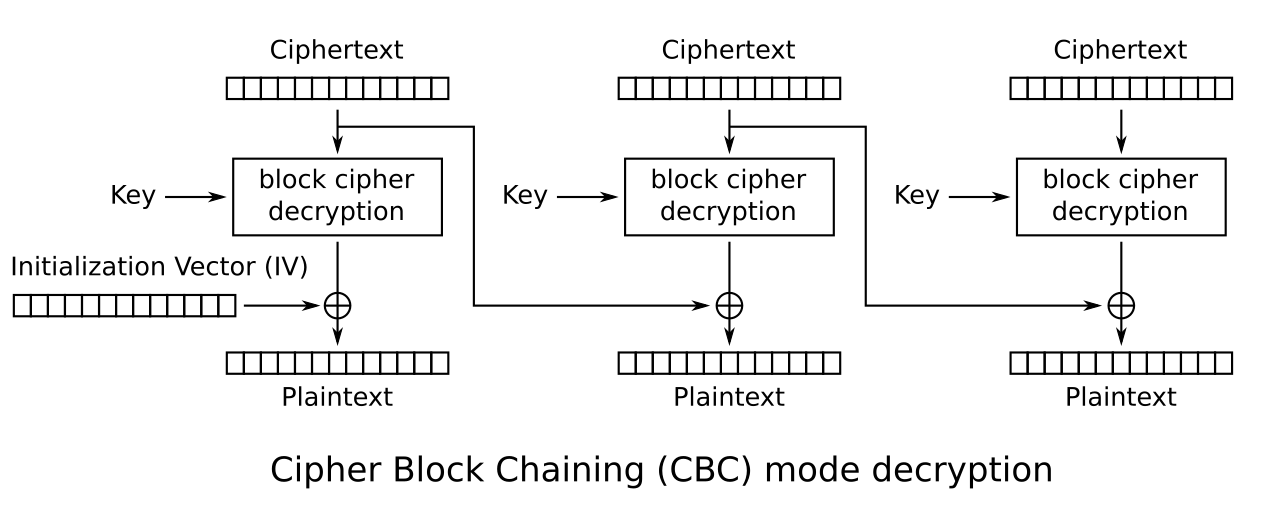
\includegraphics[width=0.92\textwidth]{images/cbc_decryption.png}
    \caption{CBC decryption in block chaining mode. The XOR with the previous ciphertext block is the property that padding oracle attacks exploit.}
    \caption*{\footnotesize Source: Wikimedia Commons, \emph{CBC decryption.svg} (public domain).}
    \label{fig:cbc-overview}
\end{figure}

In a normal passive setting, CBC can hide the plaintext content effectively when the IV is random and the key remains secret. The difficulty begins when the attacker can tamper with the ciphertext. Because $P_i$ is produced by XORing $D_K(C_i)$ with $C_{i-1}$, changing bytes in $C_{i-1}$ predictably changes bytes in the decrypted block $P_i$. The attacker still does not know $D_K(C_i)$, but the attacker can influence the final plaintext seen by the receiver.

This property has two consequences. First, tampering with one ciphertext block corrupts the next plaintext block in a controlled way. Second, if the receiver exposes any property of that corrupted plaintext, such as whether the padding is syntactically valid, the attacker can transform this malleability into a decryption attack. CBC therefore provides no built-in integrity protection. It must be combined with authentication to resist active attacks.

\section{PKCS\#7 Padding and Padding Validation}

AES operates on 16-byte blocks, but real messages are rarely an exact multiple of 16 bytes. Padding solves this mismatch by extending the message to the next block boundary. In PKCS\#7 padding, if $k$ bytes are needed, then the sender appends $k$ copies of the byte value $k$. The receiver decrypts the final block, reads the last byte, and checks whether the last $k$ bytes are all equal to $k$.

\begin{figure}[H]
    \centering
    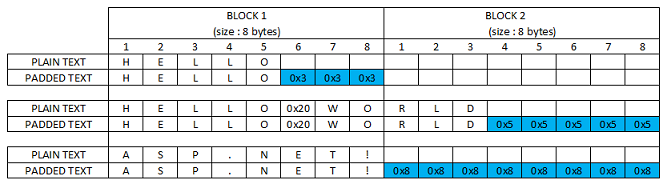
\includegraphics[width=0.8\textwidth]{images/pkcs7_padding.png}
    \caption{Example of PKCS\#7 padding patterns for different message lengths.}
    \caption*{\footnotesize Source: Bilgehanturan, Wikimedia Commons, \emph{Padding en.png} (CC BY-SA 4.0).}
    \label{fig:pkcs7}
\end{figure}

The padding rule itself is straightforward. The security issue appears during decryption. If the last byte claims that the padding length is 4, then the receiver must verify that the last four bytes are all equal to \texttt{04}. If they are not, the receiver rejects the ciphertext. From a software-engineering point of view, this validation seems harmless. From a cryptographic point of view, it can be dangerous because the rejection leaks information about the decrypted plaintext.

The key observation is that the attacker does not need a detailed error message. A single-bit answer is enough:

\begin{center}
\textit{``Did the modified ciphertext produce valid padding: yes or no?''}
\end{center}

That bit may leak through an explicit error page, a protocol alert, a timing difference, a dropped connection, or a change in application behavior. Once the attacker can distinguish valid padding from invalid padding, the receiver has effectively become a padding oracle.

The padding check is therefore not the root problem by itself. The real problem is the combination of three properties:

\begin{itemize}
    \item CBC malleability,
    \item unauthenticated decryption, and
    \item observable validation behavior.
\end{itemize}

When these three properties coexist, the attacker can learn plaintext without ever recovering the secret key.

\section{Padding Oracle Attack Model}

In a padding oracle attack, the attacker is assumed to be active on the communication path. The attacker can intercept ciphertext, alter selected bytes, submit the modified ciphertext to the target system, and observe the target's response. This makes the attack a chosen-ciphertext attack rather than a passive attack on captured data.

The oracle does not need to reveal the plaintext, the key, or even a detailed parsing error. It only needs to distinguish between ``valid'' and ``invalid'' outcomes after decryption. Formally, the oracle can be modeled as a function

\[
\mathcal{O}(C') =
\begin{cases}
1 & \text{if decrypted padding is valid,} \\
0 & \text{otherwise.}
\end{cases}
\]

Here $C'$ is a ciphertext chosen by the attacker. The attacker uses the answer to test hypotheses about the decrypted block.

The typical target is a two-block fragment: the attacker chooses a forged block $C'_{i-1}$ and appends the real ciphertext block $C_i$. The receiver decrypts $C_i$ normally, XORs the result with the forged previous block, and then performs padding validation on the resulting plaintext block. The attacker never sees that plaintext block directly, but the oracle reveals whether it ends with a valid padding pattern.

This attack model is powerful because it converts a very small side channel into a decryption tool. If a server validates padding before authenticating the message, or if the server exposes different behavior for different types of failure, then each oracle query gives the attacker information. Repeating the process across many guesses lets the attacker recover the whole message block by block.

\section{Core Attack Mathematics}

To express the attack cleanly, define the \emph{intermediate value}

\begin{equation}
    I_i = D_K(C_i).
\end{equation}

Then CBC decryption becomes

\begin{equation}
    P_i = I_i \oplus C_{i-1}.
\end{equation}

The attacker does not know $I_i$, but the attacker can replace $C_{i-1}$ by a forged block $C'_{i-1}$. The receiver will then compute

\begin{equation}
    P'_i = I_i \oplus C'_{i-1}.
\end{equation}

The attack works by choosing $C'_{i-1}$ so that the last bytes of $P'_i$ become a valid PKCS\#7 padding. When the oracle returns ``valid,'' the attacker learns a relationship between the guessed bytes in $C'_{i-1}$ and the unknown bytes of $I_i$.

\subsection{Recovering the Last Byte}

Suppose the attacker wants the last byte of $P'_i$ to equal \texttt{01}. Let the attacker guess a value $g$ for the last byte of the forged previous block. The receiver computes

\[
P'_i[16] = I_i[16] \oplus g.
\]

If the oracle returns ``valid'' for a one-byte padding, then

\[
I_i[16] \oplus g = 01,
\]

which means

\begin{equation}
    I_i[16] = g \oplus 01.
\end{equation}

Once $I_i[16]$ is known, the last byte of the original plaintext follows immediately:

\begin{equation}
    P_i[16] = I_i[16] \oplus C_{i-1}[16].
\end{equation}

\subsection{Recovering Earlier Bytes}

After recovering the final byte, the attacker moves left. To recover byte 15, the attacker first forces the last byte of $P'_i$ to become \texttt{02} and then searches for a guess that also makes byte 15 equal \texttt{02}. More generally, when recovering byte position $j$, the attacker fixes all bytes to the right of $j$ so that they decrypt to the desired padding value

\[
16 - j + 1.
\]

The process repeats until the whole block is known. On average, each byte requires around 128 oracle queries because there are 256 possibilities for a byte and only one correct value is expected.

\subsection{Small Dry Run Example}

The abstract equations become much easier to follow with one fixed example. Assume AES has a 16-byte block size and the attacker submits \emph{two ciphertext blocks} to the oracle:

\[
C'_{i-1} \,\|\, C_i
\]

Here $C_i$ is the target block kept unchanged, while $C'_{i-1}$ is the forged previous block chosen by the attacker. The oracle decrypts $C_i$, XORs it with $C'_{i-1}$, and only tells the attacker whether the result ends with valid padding.

For explanation purposes, suppose the \emph{real} plaintext of the target block is

\[
P_i = \texttt{Meet me at dawn!}
\]

which is exactly 16 bytes, so it fills one block:

\begin{center}
\texttt{4D 65 65 74 20 6D 65 20 61 74 20 64 61 77 6E 21}
\end{center}

Assume the original previous ciphertext block ends with

\begin{center}
\texttt{... 5C A5}
\end{center}

so the last two plaintext bytes are

\begin{center}
\texttt{6E 21 = "n!"}
\end{center}

The attacker does not know these values during the real attack. They are shown here only to make the dry run understandable.

\begin{table}[H]
    \centering
    \caption{Setup for the dry-run example}
    \label{tab:dry-run-setup}
    \begin{tabular}{@{}p{0.28\textwidth}p{0.62\textwidth}@{}}
        \toprule
        Item & Value \\
        \midrule
        Block size & 16 bytes \\
        Ciphertext sent to oracle & forged block $C'_{i-1}$ followed by fixed block $C_i$ \\
        Text form of $P_i$ & \texttt{Meet me at dawn!} \\
        Last two bytes of $C_{i-1}$ & \texttt{5C A5} \\
        Last two bytes of $P_i$ & \texttt{6E 21} = \texttt{n!} \\
        \bottomrule
    \end{tabular}
\end{table}

\begin{table}[H]
    \centering
    \caption{CBC view of the same example}
    \label{tab:dry-run-diagram}
    \begin{tabular}{@{}p{0.22\textwidth}p{0.22\textwidth}p{0.16\textwidth}p{0.28\textwidth}@{}}
        \toprule
        Stage & Previous block & Target block & Result suffix \\
        \midrule
        Original message & \texttt{... 5C A5} & \texttt{$C_i$} & \texttt{6E 21} = \texttt{n!} \\
        Last-byte attack & \texttt{... ?? 85} & \texttt{$C_i$} & \texttt{?? 01} \\
        Two-byte attack & \texttt{... 30 86} & \texttt{$C_i$} & \texttt{02 02} \\
        \bottomrule
    \end{tabular}
\end{table}

\paragraph{What stays fixed and what changes?}
The target block $C_i$ never changes. The attacker only changes the previous block. Because CBC decryption uses

\[
P'_i = D_K(C_i) \oplus C'_{i-1},
\]

changing $C'_{i-1}$ changes the plaintext that appears after decryption. The oracle does not reveal the plaintext directly. It only says whether the last bytes form valid padding.

\paragraph{Step 1: Recover byte 16.}
To recover the last plaintext byte, the attacker wants the final decrypted byte to become \texttt{01}, because \texttt{01} is valid PKCS\#7 padding.

Suppose the attacker tries a forged last byte

\[
C'_{i-1}[16] = \texttt{85}.
\]

Assume the oracle now returns \texttt{valid}. That means the last byte of the decrypted block became \texttt{01}. In symbols,

\[
I_i[16] \oplus \texttt{85} = \texttt{01}.
\]

Therefore,

\[
I_i[16] = \texttt{85} \oplus \texttt{01} = \texttt{84}.
\]

Now the attacker recovers the original last plaintext byte using the \emph{original} previous block byte \texttt{A5}:

\[
P_i[16] = I_i[16] \oplus C_{i-1}[16]
        = \texttt{84} \oplus \texttt{A5}
        = \texttt{21}.
\]

Hex \texttt{21} is the character \texttt{!}. So the attacker has recovered the last byte of the real plaintext.

\paragraph{Step 2: Recover byte 15.}
Now the attacker wants the last \emph{two} bytes of the forged plaintext to become \texttt{02 02}.

The last byte is already solved, so the attacker first forces byte 16 to decrypt to \texttt{02}:

\[
C'_{i-1}[16] = I_i[16] \oplus \texttt{02}
             = \texttt{84} \oplus \texttt{02}
             = \texttt{86}.
\]

Next the attacker guesses byte 15 of the forged block. Suppose the oracle returns \texttt{valid} when

\[
C'_{i-1}[15] = \texttt{30}.
\]

Then byte 15 of the decrypted block must be \texttt{02}, so

\[
I_i[15] \oplus \texttt{30} = \texttt{02}.
\]

Thus

\[
I_i[15] = \texttt{30} \oplus \texttt{02} = \texttt{32}.
\]

Now the attacker uses the original byte \texttt{5C} from $C_{i-1}$:

\[
P_i[15] = I_i[15] \oplus C_{i-1}[15]
        = \texttt{32} \oplus \texttt{5C}
        = \texttt{6E}.
\]

Hex \texttt{6E} is the character \texttt{n}. So the attacker has now recovered the last two plaintext bytes:

\begin{center}
\texttt{6E 21 = "n!"}
\end{center}

This is the key idea of the attack. The attacker never decrypts $C_i$ directly and never learns the key. Instead, the attacker learns one byte at a time by forcing valid padding patterns and using XOR to recover the original plaintext.

\subsection{Complexity and Practical Meaning}

The attack does not recover the key, yet it still defeats confidentiality. For an $n$-block message, the attacker can recover the plaintext with a manageable number of oracle queries. The exact cost depends on implementation details and the amount of retry logic available to the attacker, but conceptually the attack is efficient enough to be practical when the target system accepts repeated modified ciphertexts.

This is the main mathematical lesson of the project: the attacker is not breaking AES. The attacker is exploiting the algebra of CBC decryption together with a validation side channel.

\section{POODLE as the Main Case Study}

POODLE stands for \emph{Padding Oracle On Downgraded Legacy Encryption}. The attack became public in 2014 and demonstrated that SSL 3.0 was no longer acceptable for modern secure communication. Its importance goes beyond one protocol version. POODLE showed how an old protocol, compatibility fallbacks, and CBC padding behavior can combine into a practical attack against real users.

The key setting was the downgrade path. Many clients and servers still supported SSL 3.0 for backward compatibility, and some clients would fall back to SSL 3.0 if earlier handshake attempts failed. A man-in-the-middle attacker could interfere with the connection, trigger the fallback, and force the victim to communicate under SSL 3.0. Once that happened, the attacker could exploit SSL 3.0's CBC record processing.

The SSL 3.0 design was especially weak because the padding bytes were not constrained the way later TLS versions intended. In SSL 3.0, only the padding length byte had a strict meaning, while the other padding bytes could be arbitrary. As a result, a modified record could accidentally satisfy the padding format with probability about $1/256$ for a targeted byte. That probability is small for a single attempt but becomes practical when the attacker can trigger many repeated requests carrying a secret such as a session cookie.

\begin{figure}[H]
    \centering
    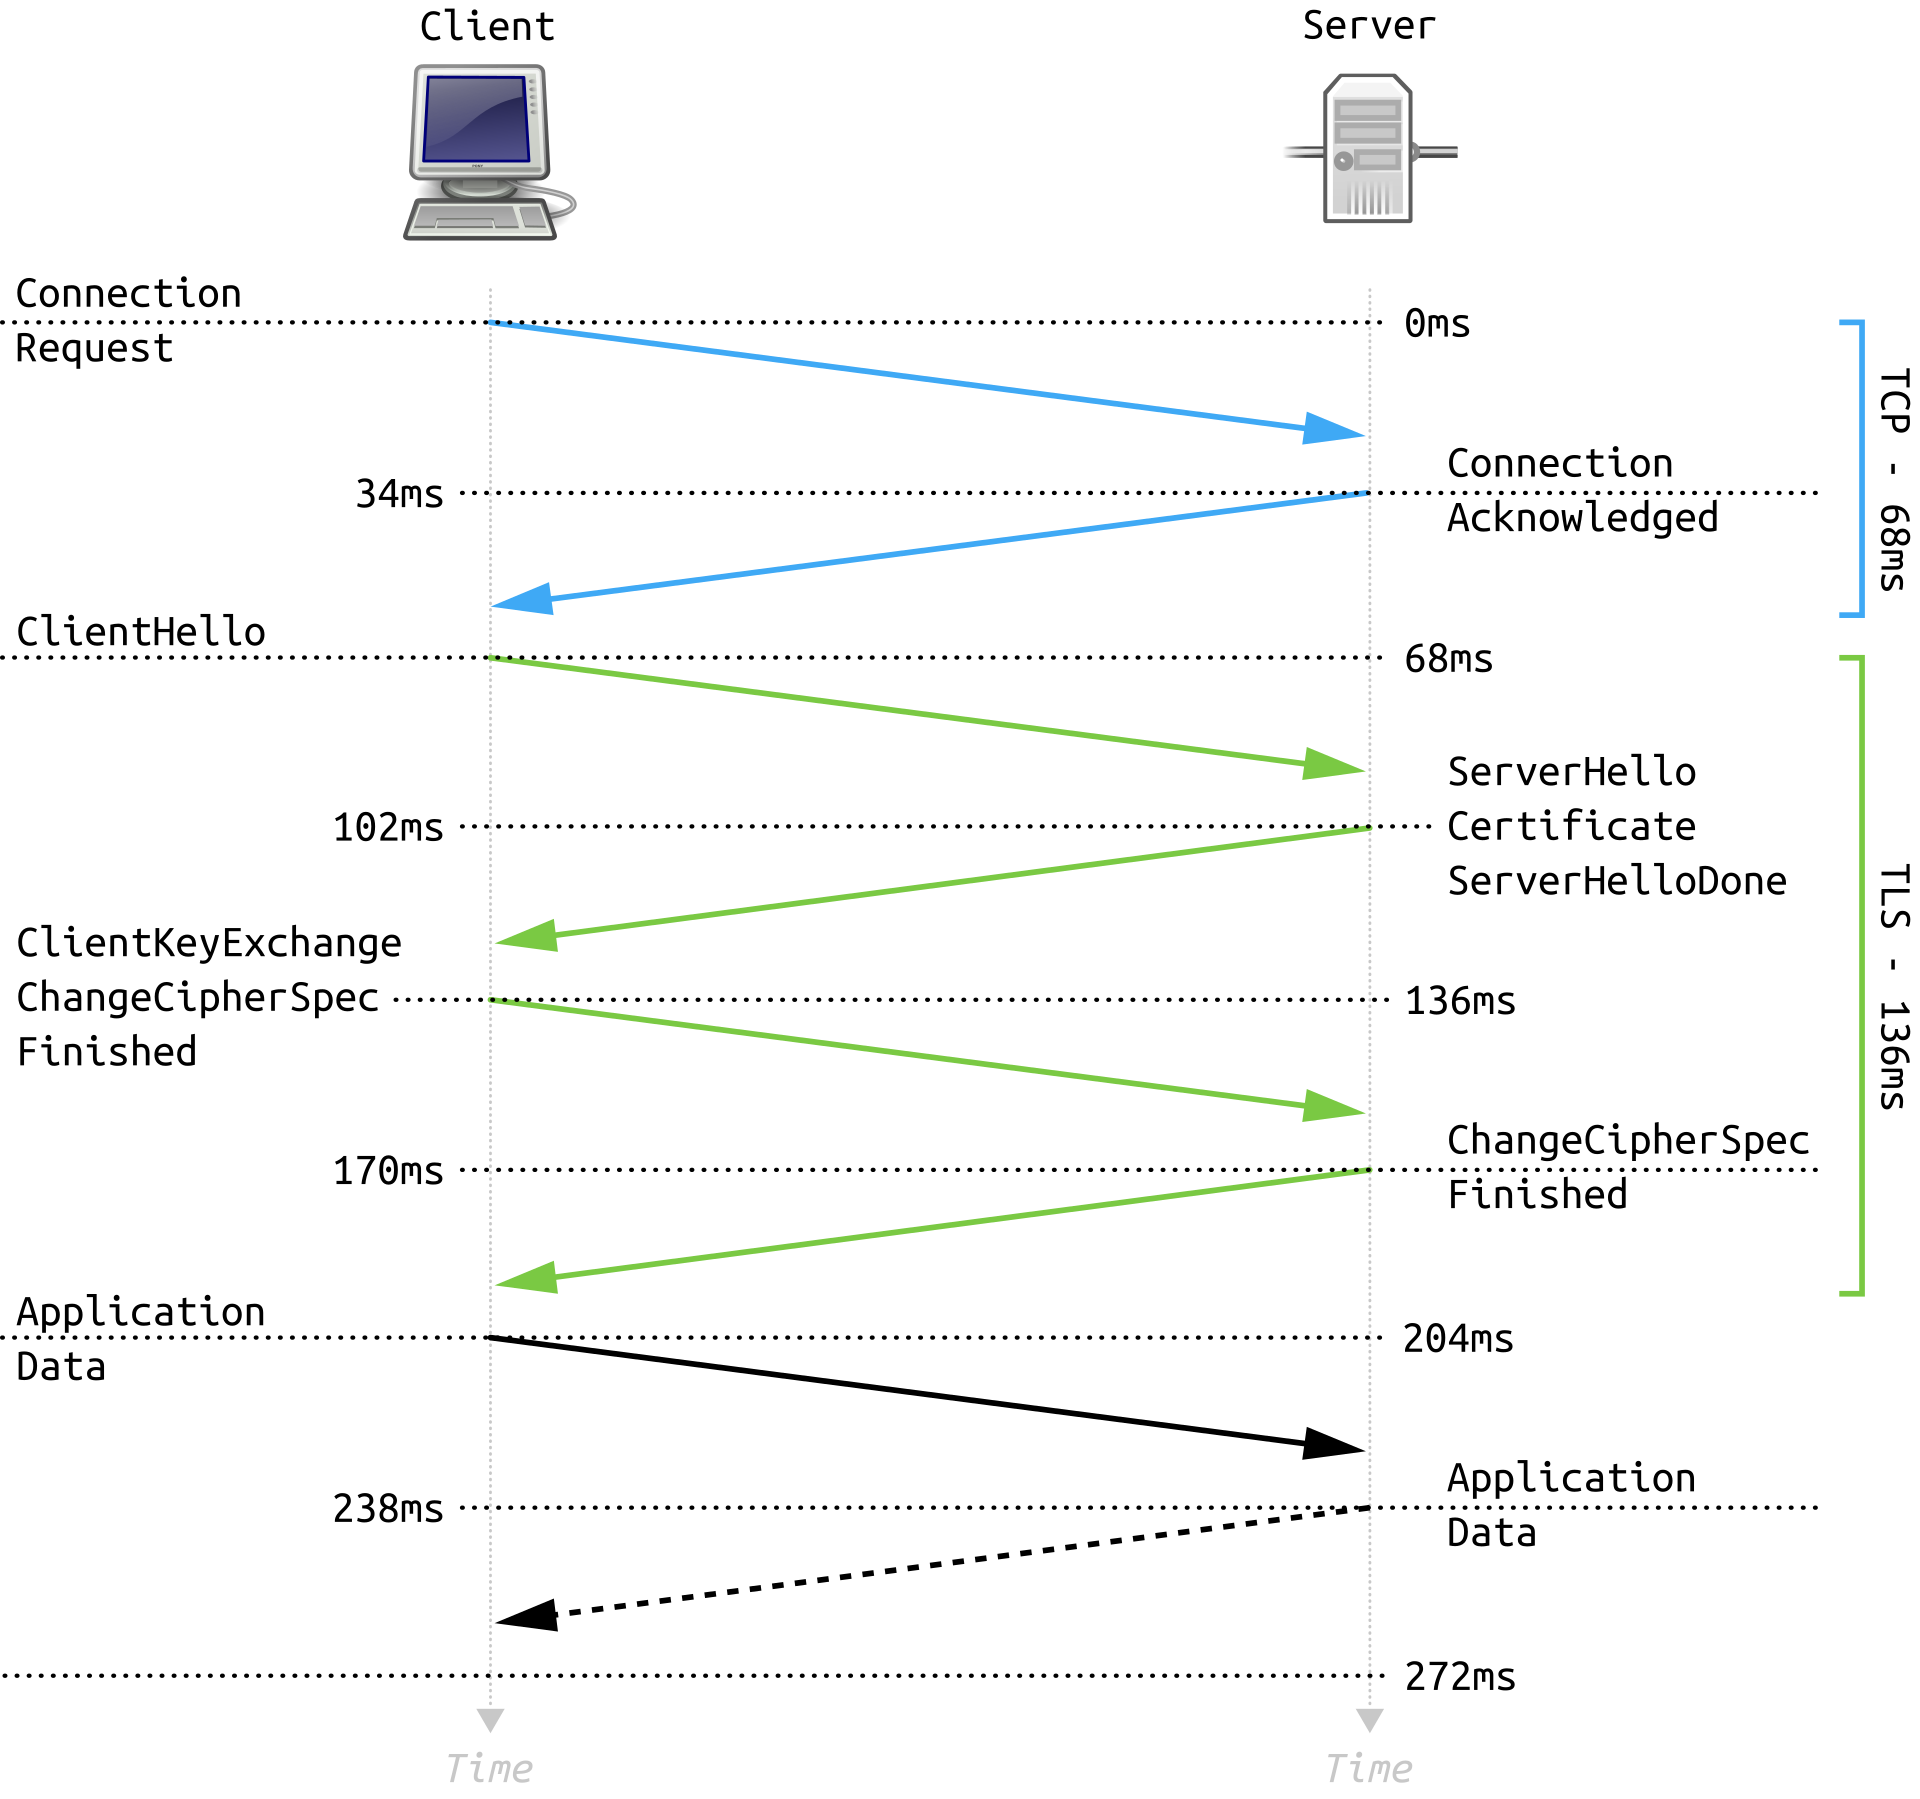
\includegraphics[width=0.78\textwidth]{images/tls12_handshake.png}
    \caption{Handshake message flow in the TLS protocol family. POODLE targeted the older SSL 3.0 branch of this protocol line through downgrade and CBC-padding weaknesses.}
    \caption*{\footnotesize Source: Wikimedia Commons, \emph{Full TLS 1.2 Handshake.svg}.}
    \label{fig:ssl-simple}
\end{figure}

The attack workflow can be summarized as follows:

\begin{enumerate}
    \item the attacker forces a downgrade from a newer protocol to SSL 3.0,
    \item the attacker causes the victim to send repeated requests containing a secret value,
    \item the attacker manipulates ciphertext blocks in those requests, and
    \item the server's acceptance or rejection of the padding reveals one byte of information at a time.
\end{enumerate}

POODLE therefore turned a theoretical padding oracle into a network attack against web traffic. It also changed operational practice. After the disclosure, major vendors disabled SSL 3.0 support, and the IETF formally deprecated SSL 3.0. The lesson was not only that legacy protocols are dangerous, but also that backward-compatibility paths can revive vulnerabilities long after the community believes it has moved on.

It is important to distinguish POODLE from the local Python demonstration in this project. The project code demonstrates the \emph{generic padding oracle mechanism}: forged ciphertext, padding validation, and byte-by-byte plaintext recovery. POODLE adds protocol-specific details such as downgrade behavior, repeated browser requests, and SSL 3.0 record semantics. The mathematical core is shared, but the surrounding attack environment is richer in the real protocol case.

\section{Why the Attack Works in Practice}

At first sight, a single valid-or-invalid bit seems too weak to reveal a message. In practice, it is enough because the attacker controls the input and can repeat the experiment many times. Each oracle query tests one hypothesis about the decrypted bytes. Over hundreds or thousands of such tests, the attacker gradually reduces uncertainty until the plaintext is known.

Several engineering decisions make this possible:

\begin{itemize}
    \item \textbf{Unauthenticated decryption.} The receiver decrypts before confirming that the ciphertext is genuine.
    \item \textbf{Distinguishable failures.} Padding errors, MAC errors, connection aborts, or timing differences reveal different outcomes.
    \item \textbf{Retry opportunities.} Web requests, API calls, or protocol handshakes can often be repeated many times.
    \item \textbf{Predictable secret placement.} Cookies, tokens, and structured messages often appear at stable positions in encrypted records.
\end{itemize}

Another practical point is that not all padding oracles look the same. Some systems leak the oracle directly through an explicit error. Others leak it indirectly through elapsed time or subtle changes in code path. Lucky13 is a classic example of a related CBC attack where timing differences during MAC and padding processing were enough to create a side channel. Lucky13 is not the main topic of this report, but it reinforces the same design lesson: decryption behavior itself can become a leakage source.

The attack also works because the adversary can manipulate one block to learn about the next block. This means a protocol does not need to reveal the entire decrypted message. Even small fragments of post-decryption logic can be enough. A parser rejecting malformed padding, a web application returning a different error page, or a TLS implementation taking a slightly different amount of time may all act as an oracle.

In other words, the attack succeeds not because the underlying block cipher is weak, but because the surrounding system leaks information after decryption and before the ciphertext is authenticated.

\section{Brief Implementation Overview of the Python Demo}

To support the theoretical discussion, the project includes a compact Python demonstration. The implementation is intentionally local and simplified so that the attack can be observed step by step in a terminal.

\begin{table}[H]
    \centering
    \caption{Implementation stack used in the project demonstration}
    \label{tab:implementation-stack}
    \begin{tabular}{@{}ll@{}}
        \toprule
        Component & Choice \\
        \midrule
        Programming language & Python 3 \\
        Symmetric cipher library & PyCryptodome \\
        Networking framework & Flask + HTTP requests \\
        Mode of operation & AES-128-CBC \\
        Padding scheme & PKCS\#7 \\
        Demonstration style & Local terminal-based CBC oracle demo \\
        \bottomrule
    \end{tabular}
\end{table}

The server script plays two roles. First, it encrypts user-provided plaintext under AES-CBC with a random IV. Second, it exposes an oracle endpoint that answers a very narrow question: whether the decrypted final block has valid PKCS\#7 padding. This models the vulnerable system.

The attacker script receives the ciphertext, splits it into blocks, and attacks one target block at a time. For each byte position, the script forges a previous block, submits candidate ciphertexts to the oracle, and checks which candidate produces valid padding. When that happens, the script computes the corresponding intermediate byte and then the original plaintext byte. The process repeats from right to left until the entire plaintext is recovered.

This implementation demonstrates the core idea clearly:

\begin{itemize}
    \item the attacker never uses the encryption key,
    \item the attacker does not decrypt the target block directly,
    \item the only information leaked by the oracle is padding validity, and
    \item that single bit is still sufficient to recover plaintext.
\end{itemize}

The demo is not a complete reproduction of POODLE. It does not model browser fallback, real SSL 3.0 records, or web cookie extraction. Instead, it isolates the algebra and oracle behavior that make the broader family of attacks possible. This makes it suitable for classroom demonstration, report discussion, and viva explanation.

If the project were extended, tools such as Burp Suite could be added to observe or manipulate traffic in a web setting. For the current submission, the Python demo is enough to show the cryptographic weakness directly.

\section{Defenses and Current Industry Practice}

Padding oracle attacks are prevented by stopping the receiver from giving useful feedback on modified ciphertext. The safest solution is to use authenticated encryption instead of plain CBC encryption.

\begin{itemize}
    \item \textbf{Use authenticated encryption.} Modes such as AES-GCM and ChaCha20-Poly1305 provide both confidentiality and integrity. This means the message is not only encrypted, but also checked to see whether anyone changed it.
    \item \textbf{Reject modified ciphertext early.} If authentication fails, the system should stop immediately. It should not continue to padding checks or reveal anything about the decrypted message.
    \item \textbf{Do not rely on CBC alone.} CBC can hide data from a passive attacker, but it does not stop an active attacker from modifying ciphertext blocks. That is why CBC by itself is not enough for secure communication.
    \item \textbf{Keep failure behavior uniform.} The system should not leak useful differences through error messages, timing, or connection behavior. All failures should look as similar as possible so that attackers cannot learn anything from the response.
\end{itemize}

In practice, this leads to the following recommendations:

\begin{itemize}
    \item disable SSL 3.0,
    \item avoid old CBC-based cipher suites,
    \item use TLS 1.3 whenever possible,
    \item if TLS 1.2 must be used, prefer AEAD suites such as AES-GCM or ChaCha20-Poly1305,
    \item treat constant-time processing and uniform errors as extra protection, not the main fix.
\end{itemize}

Current industry practice is based on these lessons:

\begin{itemize}
    \item SSL 3.0 is deprecated,
    \item TLS 1.0 and TLS 1.1 are also deprecated,
    \item TLS 1.3 uses modern authenticated encryption,
    \item modern secure systems prefer AEAD-based designs instead of CBC with padding checks.
\end{itemize}

The main lesson is simple: \textbf{encryption alone is not enough}. Modern systems combine confidentiality and integrity so that attackers cannot learn anything useful by modifying ciphertext.

\section{Learning Outcomes and Conclusion}

This project leads to several important learning outcomes. First, CBC mode is easy to understand algebraically, but that same algebra explains why active tampering is dangerous. Second, padding is not just a formatting detail. Once padding validation becomes visible to an attacker, it becomes a cryptographic side channel. Third, chosen-ciphertext attacks can be devastating even when the attacker never obtains the key and never sees the plaintext directly.

POODLE provides the real-world lesson. A combination of legacy protocol support, downgrade behavior, and weak CBC padding handling turned a subtle theoretical issue into a serious web security problem. The local Python demonstration then shows the same logic in a controlled way: modify a previous block, ask the oracle whether padding is valid, and recover bytes one by one.

The final conclusion is that classic encryption without authentication is not sufficient for modern secure systems. CBC mode by itself does not stop an active attacker from tampering with ciphertext. The correct modern answer is authenticated encryption, careful protocol design, and the removal of obsolete fallback behavior. That is why current practice favors AEAD-based protocols and why old CBC padding failures remain an important topic in applied cryptography education.


\end{document}
